\section{OpenMP parallelization and execution analysis: Jacobi}
\subsection{Parallelization}
\justify
The first algorithm that we parallelize is Jacobi's. In order to do that, the first thing we do is to distribute the work among the threads based on the data. We followed a geometric data block decomposition model; which means that the data is split into equal and consecutive blocks and each block is given to one processor. If the size of data can be expressed by N and the number of threads P, each block's size is N/P.
\justify
\begin{figure}[h!]
    \centering
    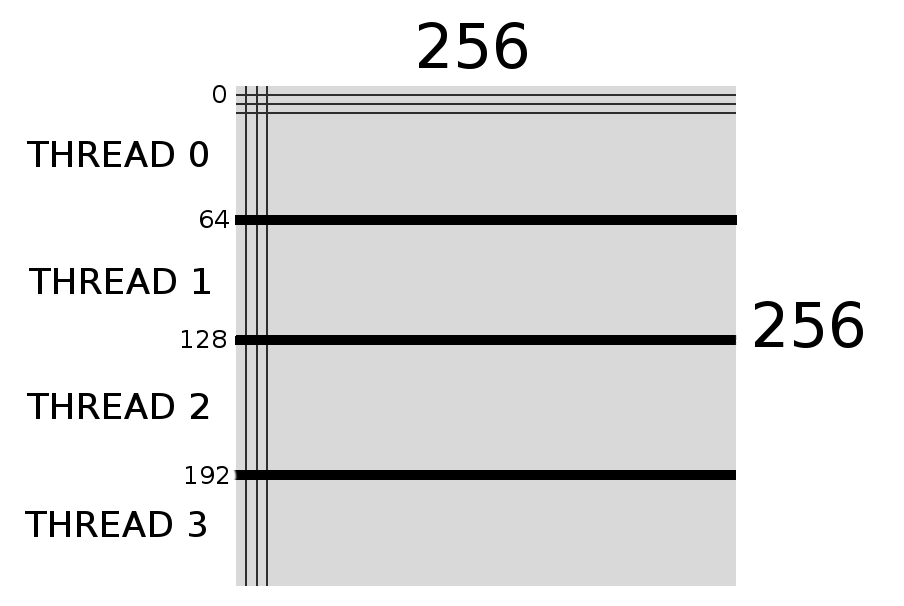
\includegraphics[width=0.5\textwidth]{distribution.png}
    \caption{Diagram of geometric block data distribution}
    \label{fig:dist}
\end{figure}
\justify
In this particular problem, we decided to create this blocks by consecutive rows. For example and as you can see in the figure, if the matrix is 256x256 elements and we have 4 threads, one will do rows 0 to 63; the next one 64 to 127, etc...
\justify
To accomplish this, we use the macros that are given to us to calculate these boundaries. When the main program arrives to the parallel region, it divdes into several threads. Since the original code defines the variable \textit{howmany} as the number of data blocks, we keep using it instead of making as many blocks as threads. Each thread calculates its boundaries based on its thread id and then jumps into the for loops; which start and end limits are based on the boundaries calculated before. You can see this implementation on the code below.
\clearpage
\begin{lstlisting}

double relax_jacobi (double *u, double *utmp, unsigned sizex, 
unsigned sizey)
{
  double  sum=0.0;
  #pragma omp parallel reduction(+:sum)
  {
    int howmany=4;
    if(howmany>omp_get_num_threads())howmany=omp_get_num_threads();
    //for (int blockid = 0; blockid < howmany; ++blockid) {
    int blockid = omp_get_thread_num();
    int i_start = lowerb(blockid, howmany, sizex);
    int i_end = upperb(blockid, howmany, sizex);
    for (int i=max(1, i_start); i<= min(sizex-2, i_end); i++) {
      for (int j=1; j<= sizey-2; j++) {
        utmp[i*sizey+j]= 0.25 * ( u[i*sizey+ (j-1) ]+ // left
				u[i*sizey + (j+1)]+  // right
				u[ (i-1)*sizey + j]+  // top
				u[ (i+1)*sizey + j]); // bottom
        double diff;	
        diff = utmp[i*sizey+j] - u[i*sizey + j];
        sum += diff * diff; 
	  }
	}
	//}
  }
  return sum;
}
\end{lstlisting}
\justify
The variable sum encounters a data-race problem as several threads are reading and writting its value; so we decided to fix it in the easiest way possible making it a reduction. Another problem was the variable diff, which was declared in the same line as the variable sum and therefore would be shared among threads. We could have made it private in the parallel region declaration but we decided to move the variable declaration inside the region; making it local to each thread.
\justify
\subsection{Performance Evaluation}
\justify
Once we tested that the parallel version gives a correct output (comparing the image to the sequential one), we evaluated the speed-up. First, we compared the execution time of both sequential and parallel version and obtained that the first one lasted 5.219s with 2142.62 MFlop/s and the second one 3.235s with 3456.07 MFlop/s. This means a speed-up of 1.613.
\clearpage
\justify
Another measure to evaluate the performance is the strong-scallability plot.
\begin{figure}[h!]
    \centering
    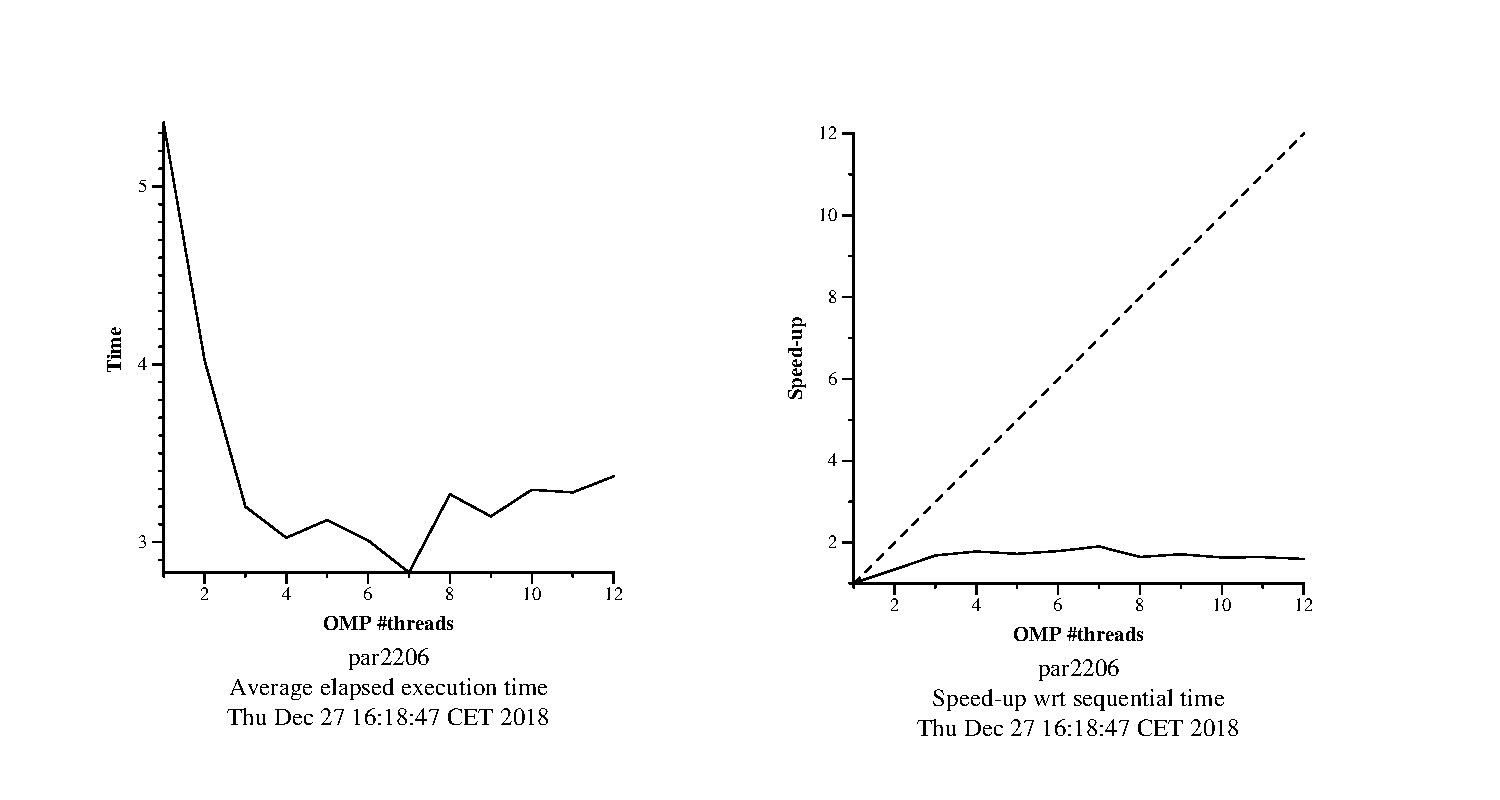
\includegraphics[width=0.99\textwidth]{jacobi-strong-howmany.png}
    \caption{Jacobi strong scallabilty speed-up plots}
    \label{fig:stronghowmany}
\end{figure}
\justify
As it can be easily seen in the figure, the scallability is really far from ideal. This is in part due to the implicit limitation in keeping the \textit{howmany} variable. We are limiting the maximum number of blocks to 4, and in consequence only 4 threads are going to work at maximum, as you can see in the figure below where we only show one iteration (one call to the Jacobi function).
\begin{figure}[h!]
    \centering
    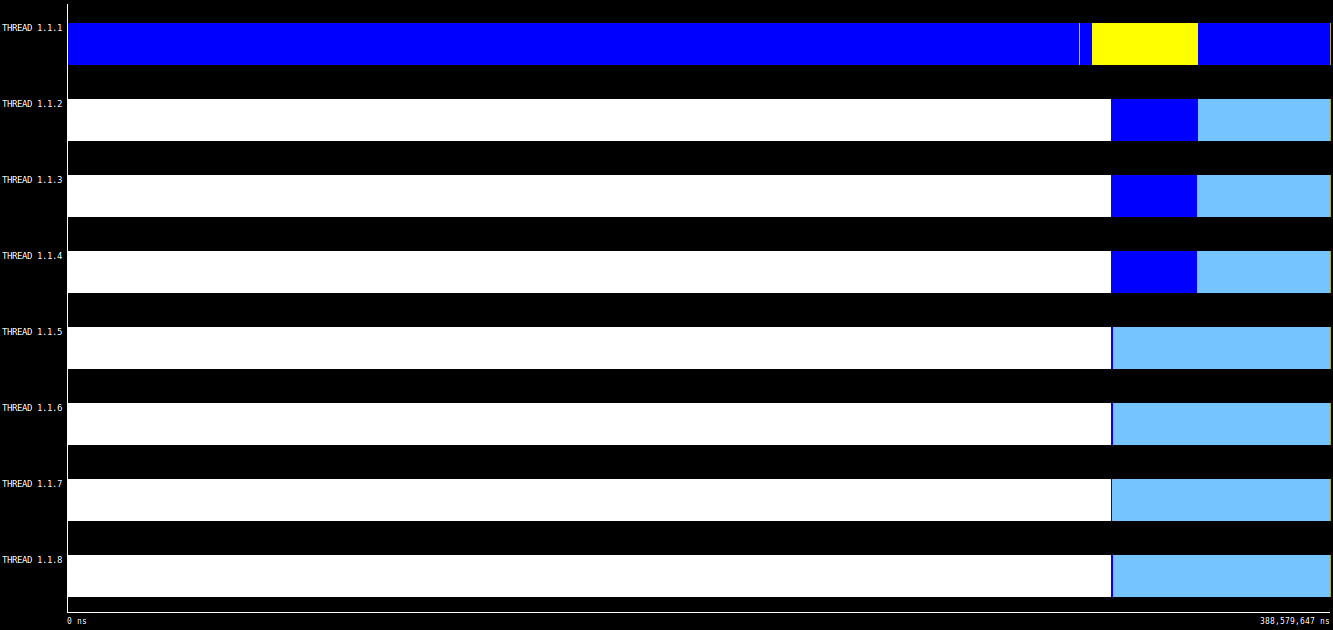
\includegraphics[width=0.80\textwidth]{howmany.png}
    \caption{Work distribution on one iteration with howmany=4}
    \label{fig:howmany}
\end{figure}
\justify
It can be seen that only 4 threads are doing real work while the other 4 wait.
\justify
In order to really evaluate the potential parallelism, we are going to remove this limitation and set the number of blocks as the number of threads in the parallel region.
\begin{lstlisting}
int howmany = omp_get_num_threads();
\end{lstlisting}
\justify
With this improvement, the new execution time is 2.845s and 3930.71 MFlop/s. Now the gain is 1.834 compared to the sequential version and 1.137 compared to the previous parallel version. We can observe in the following paraver capture that we fixed the problem with useless threads.
\begin{figure}[h!]
    \centering
    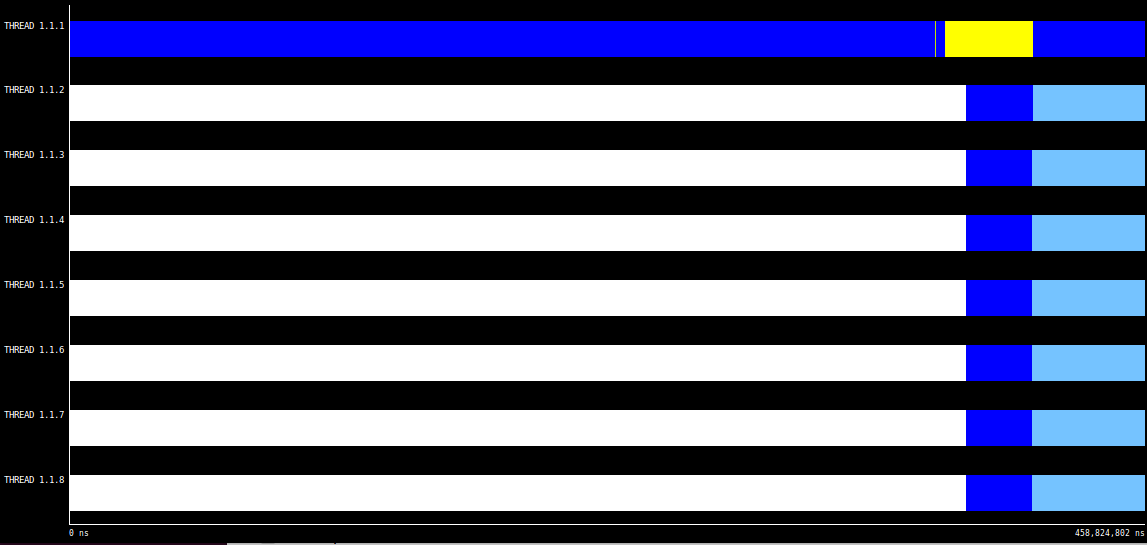
\includegraphics[width=0.80\textwidth]{improved.png}
    \caption{Work distribution on one iteration with howmany=omp\_get\_num\_threads()}
    \label{fig:howmanyyy}
\end{figure}

%\clearpage

\justify
This improvement is less notable when looking at the strong scallability plots, which are still far from ideal.
\begin{figure}[h!]
    \centering
    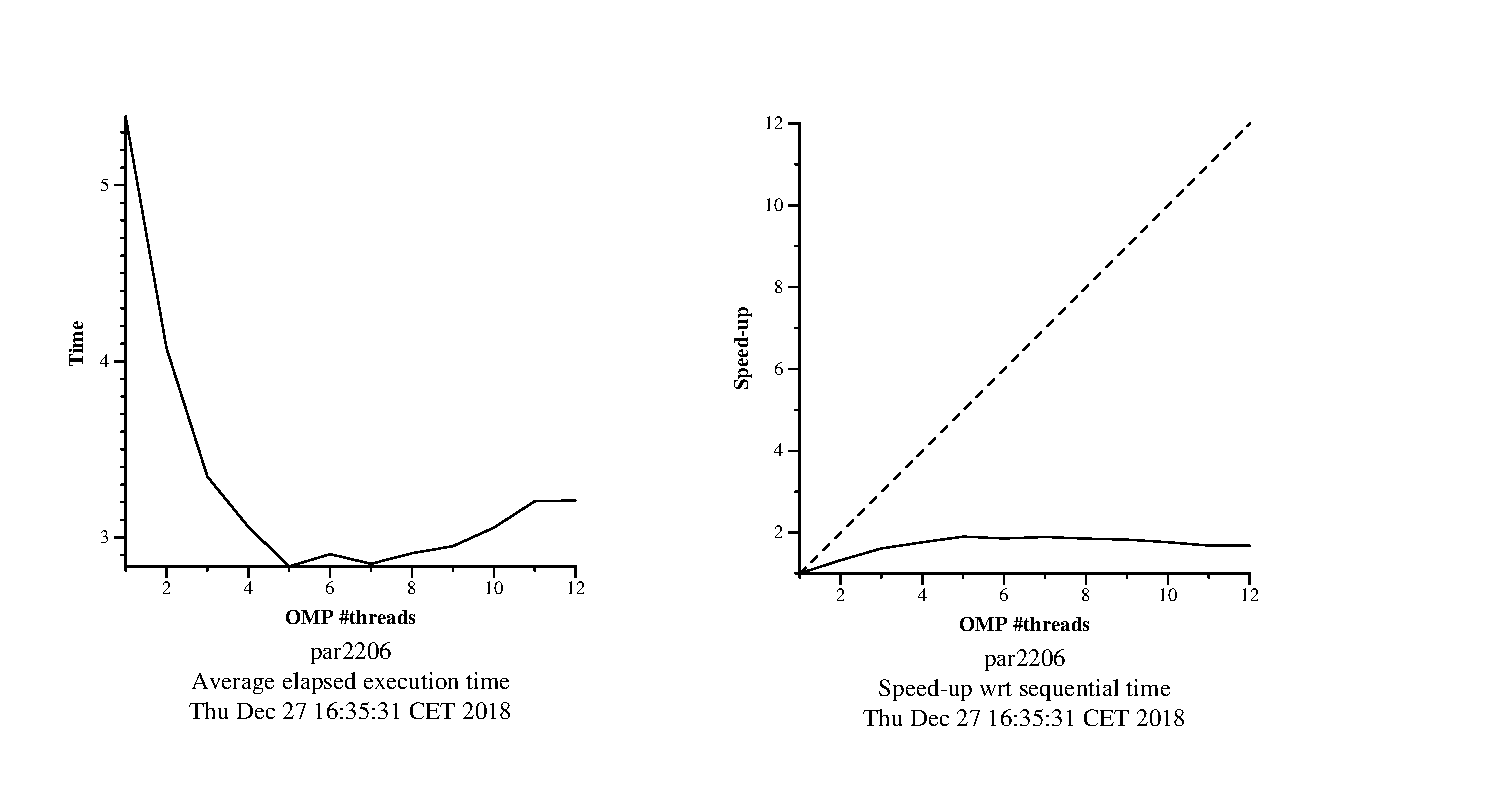
\includegraphics[width=0.99\textwidth]{jacobi-strong-improved.png}
    \caption{Jacobi improved version strong scallabilty speed-up plots}
    \label{fig:strongimproved}
\end{figure}
\justify
There's still more room for improvement in the parallelization of the Jacobi algorithm. We can see that each iteration in the main code also calls the funciton \textit{copy\_mat}. We decided to parallelize this function too following the same decomposition as the \textit{Jacobi} function :

\begin{lstlisting}
void copy_mat(double *u, double *v, unsigned sizex, unsigned sizey)
{
  #pragma omp parallel
  {
    int howmany = omp_get_num_threads(); 
    int blockid = omp_get_thread_num();
    int i_start=lowerb(blockid,howmany,sizex);
    int i_end = upperb(blockid,howmany,sizex);
    for (int i=max(1,i_start); i<=min(sizex-2,i_end); i++)
      for (int j=1; j<=sizey-2; j++) 
        v[ i*sizey+j ] = u[ i*sizey+j ];
  }
}
\end{lstlisting}

\justify
After executing this new version, we obtain an execution time of 0.852s and 13129.18 MFlop/s. This represents a gain of 6.13 compared to the sequential version (5.219s) and a gain of 3.34 compared to the last parallel version (2.845). We can put all three previous results in a table to have a better look at the improvements.

\begin{table}[!h]
\begin{tabular}{|l|l|l|l|}
\hline
Version            & Execution Time (s) & Mflops   & gain from sequential \\ \hline
Sequential         & 5.219              & 2142.62  & 1                    \\ \hline
Howmany=4          & 3.235              & 3456.07  & 1.613                \\ \hline
Removed limitation & 2.845              & 3930.71  & 1.834                \\ \hline
Copy\_mat parallel & 0.852              & 13129.18 & 6.13                 \\ \hline
\end{tabular}
\end{table}
\clearpage
\justify
This great improvement can also be seen in the following strong-scallability plots:
\begin{figure}[h!]
    \centering
    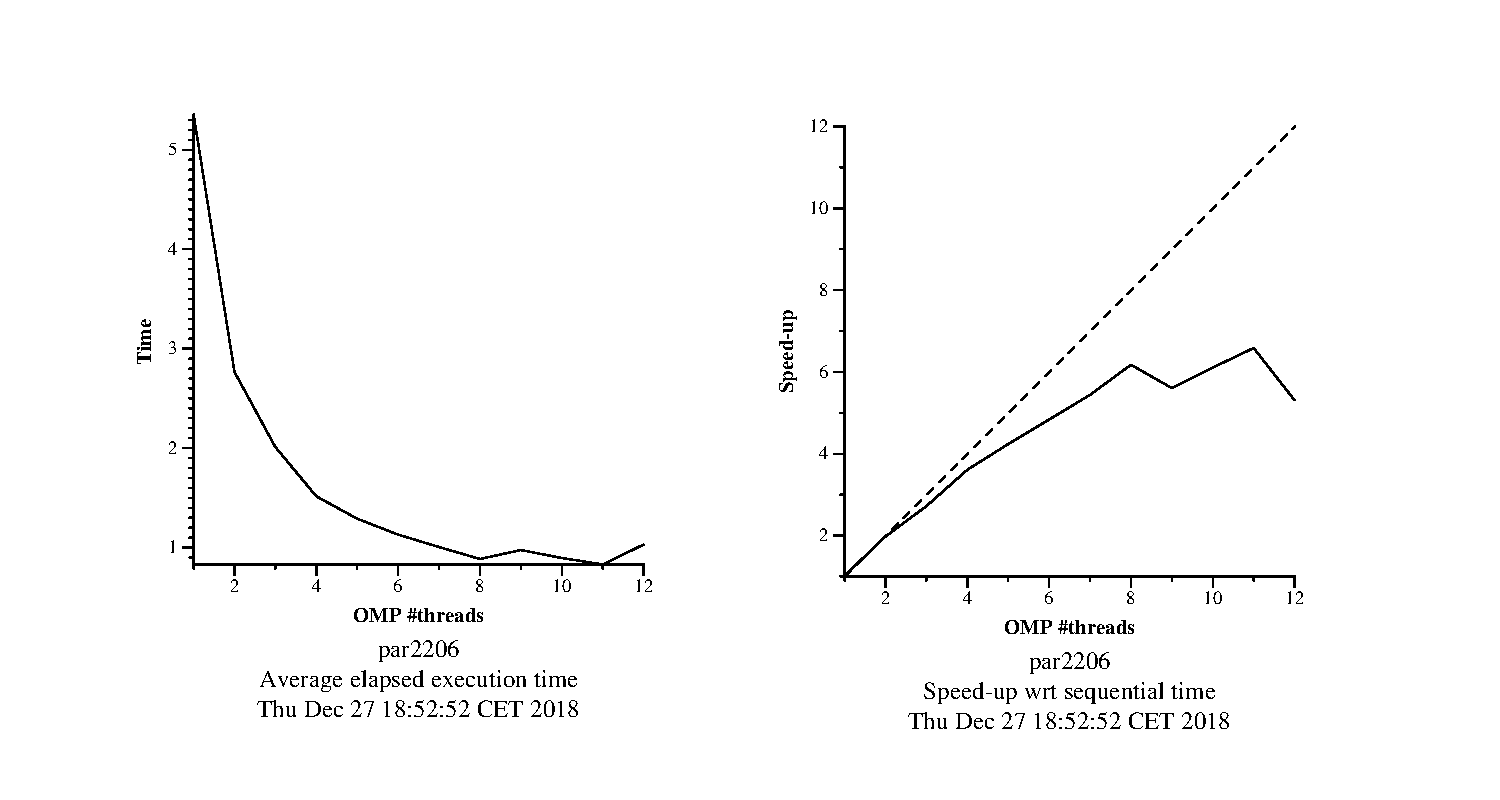
\includegraphics[width=0.99\textwidth]{improvedfinal.png}
    \caption{Jacobi final improvement version strong scallabilty speed-up plots}
    \label{fig:strongimprovedfinal}
\end{figure}